%%%%%%%%%%%%%%%%%%%%%%% file template.tex %%%%%%%%%%%%%%%%%%%%%%%%%
%
% This is a general template file for the LaTeX package SVJour3
% for Springer journals.          Springer Heidelberg 2010/09/16
%
% Copy it to a new file with a new name and use it as the basis
% for your article. Delete % signs as needed.
%
% This template includes a few options for different layouts and
% content for various journals. Please consult a previous issue of
% your journal as needed.
%
%%%%%%%%%%%%%%%%%%%%%%%%%%%%%%%%%%%%%%%%%%%%%%%%%%%%%%%%%%%%%%%%%%%

%
\RequirePackage{fix-cm}

%
\documentclass{svjour3}                     % onecolumn (standard format)
%\documentclass[smallcondensed]{svjour3}     % onecolumn (ditto)
% \documentclass[twocolumn]{svjour3}

% onecolumn (second format)
%\documentclass[twocolumn]{svjour3}          % twocolumn
%
\smartqed

% flush right qed marks, e.g. at end of proof
%
\usepackage{graphicx}

\usepackage{natbib}
\usepackage{rotating}
\usepackage{url}

\setlength\rotFPtop{0pt plus 1fil}

%
% \usepackage{mathptmx}      % use Times fonts if available on your TeX system
%
% insert here the call for the packages your document requires
%\usepackage{latexsym}
% etc.
%
% please place your own definitions here and don't use \def but
% \newcommand{}{}
%
% Insert the name of "your journal" with
\journalname{Journal of Inherited Metabolic Disease}
%
\begin{document}

\title{Estimating the probability of IQ impairment from blood phenylalanine for phenylketonuria patients%\thanks{Grants or other notes
%about the article that should go on the front page should be
%placed here. General acknowledgments should be placed at the end of the article.}
}

\subtitle{A hierarchical meta-analysis}
\titlerunning{Meta-analysis of IQ response to Phe}        % if too long for running head
\author{Christopher J. Fonnesbeck \and Melissa L. McPheeters \and Shanthi Krishnaswami \and Mary Louise Lindegren \and Tyler Reimschisel}

%\authorrunning{Short form of author list} % if too long for running head
\institute{Christopher J. Fonnesbeck \at Department of Biostatistics \\
Vanderbilt University Medical Center \\
1161 21st Ave South \\
S-2323 Medical Center North \\
Nashville, Tennessee 37232-2158 \\
Tel.: 615-936-0317 \\
\email{chris.fonnesbeck@vanderbilt.edu}
%  \\
%             \emph{Present address:} of F. Author  %  if needed
\and Melissa L. McPheeters and Shanthi Krishnaswami \at Institute for Medicine and Public Health \\
Evidence-based Practice Center \\
Vanderbilt University Medical Center \\
2525 West End Avenue, Suite 600, 6th Floor \\
Nashville, TN 37203-1738 \\
Tel.: 615.936.8317 \\
\email{melissa.mcpheeters@vanderbilt.edu}
\and Mary Louise Lindegren and Tyler Reimschisel \at Department of Pediatrics \\
Vanderbilt University Medical Center \\
2200 Children's Way \\
Nashville, TN 37232}

\date{Received: date / Accepted: date}

% The correct dates will be entered by the editor
% TODO Add word count
% TODO Add
\maketitle
\begin{abstract}
    Though the control of blood phenylalanine (Phe) levels is essential for minimizing impairment in individuals with phenylketonuria (PKU), the empirical basis for the selection of specific blood Phe levels as targets has not been evaluated. We evaluated the current evidence that particular Phe levels are optimal for minimizing or avoiding cognitive impairment in individuals with PKU. This work uses meta-estimates of blood Phe-IQ correlation to predict the probability of low IQ for a range of Phe levels. We believe this metric is easily interpretable by clinicians, and hence useful in making recommendations for Phe intake. The median baseline association of Phe with IQ was estimated to be negative, both in the context of historical (median=-0.026, 95\% BCI=[-0.040, -0.013]) and concurrent (-0.007, [-0.014, 0.000]) measurement of Phe relative to IQ. The estimated additive fixed effect of critical period Phe measurement was also nominally negative for historical measurement (-0.010, [-0.022, 0.003]) and positive for concurrent measurement (0.007, [-0.018, 0.035]). Probabilities corresponding to historical measures of blood Phe demonstrated an increasing chance of low IQ with increasing Phe, with a stronger association seen between blood Phe measured during the critical period than later. In contrast, concurrently-measured Phe was more weakly correlated with the probability of low IQ, though the correlation is still positive, irrespective of whether Phe was measured during the critical or non-critical period. This meta-analysis illustrates the utility of a Bayesian hierarchical approach for not only combining information from a set of candidate studies, but also for combining different types of data to estimate parameters of interest. \keywords{phenylketonuria \and meta-analysis \and Bayesian \and IQ \and hierarchical model}

    % \PACS{PACS code1 \and PACS code2 \and more}
    % \subclass{MSC code1 \and MSC code2 \and more}
\end{abstract}

\section{Introduction} % (fold)
\label{sec:Introduction}

Phenylketonuria (PKU) is a metabolic disorder in which a buildup of phenylalanine (Phe) in the blood results from an inability to properly metabolize that amino acid. This buildup, in turn, becomes neurotoxic and can lead to intellectual disability, delayed speech, seizures and behavioral abnormalities. PKU is typically diagnosed at birth based on newborn screening results. Approximately 1 in 13,500 to 19,000 infants in the United States is born with PKU \citep{Hegge:2009ep,NationalInstitutesofHealthConsensusDevelopmentPanel:2001ti}. The most severe form of PKU (classic PKU) is typically characterized by blood Phe levels exceeding 1200 $\mu$mol/L while on a normal diet. Individuals are diagnosed with hyperphenylalaninemia if their Phe level is above normal (120 $\mu$mol/L) but less than about 1000 $\mu$mol/L while on a normal diet (exact cutoffs vary in the literature and in practice). The mainstay for treatment of PKU is a special diet that restricts the intake of Phe in order to maintain a low Phe concentration in the blood.  With adherence to a Phe-restricted diet, adverse cognitive outcomes can be mitigated. However, management of PKU can be burdensome for the patient and their family, so there is interest in identifying alternative ways of managing this lifelong condition effectively. Further, questions remain as to the empirical basis for the selection of specific blood Phe levels as targets to reflect good dietary control.

Individuals with PKU can tolerate varying quantities of Phe intake. Their Phe levels are monitored frequently, allowing physicians to recommend appropriate modifications to Phe intake in order to determine their ideal Phe tolerance. Historically, Phe levels were only monitored closely during the first six years of life (the ``critical period") because elevated Phe was not believed to be detrimental in older individuals. However, based on accumulated evidence over the last few decades, it is now standard of care to recommend strict adherence to a Phe-restricted diet and routine monitoring of Phe levels throughout life \citep{NationalInstitutesofHealthConsensusDevelopmentPanel:2001ti, Koch:2002ul}.

In general, the treatment goal is a Phe level below 360 $\mu$mol/L, though there is some variation in the target blood Phe level between clinics and across countries \citep{NationalInstitutesofHealthConsensusDevelopmentPanel:2001ti, Giovannini:2007kg}. However, there is little empirical basis for selecting a particular Phe level as a target, and specifically, on an optimal range for minimizing the clinical and cognitive effects of hyperphenylalaninemia among individuals of varying age.

A meta-analysis by \citet{Waisbren:2007es} employed random effects models \citep{DerSimonian:1986wm} to relate IQ measurement to Phe levels, based on within-study correlations. Neuropsychological or other (non-IQ) cognitive outcomes were deemed by the authors to be too disparate to combine. Of the studies included in the analysis, only 40 presented within-study correlations and could be used in the quantitative meta-analysis. A weakness of this review is that there was no accounting for the variance of the within-study correlations for each study. This ignores a potentially important source of variation, and likely results in overly-precise meta-estimates.

In a separate, more recent meta-analysis, \citet{Albrecht:2009fb} examined the evidence for neuropsychological effects varying with Phe concentration. They restricted their meta-analysis to studies where response data were collected with computer-based measurement devices (942 individuals in total), and where PKU subjects were compared to healthy controls. The reaction time for any of a suite of neuropsychological tests was the chosen response variable. Seven different classes of test were used across studies, and combined in the meta-analysis using a standardized effect size measure \citep{Rosenthal:1994vc}. Results suggested that age was an important covariate, along with Phe and interactions of Phe with age and Phe with test type. Though no estimate of maximum Phe intake could be obtained for adults, the authors estimated an upper threshold of 320 $\mu$mol/L for children (7-13 years) and 570 $\mu$mol/L for adolescents (14-18 years).

Here, we seek to evaluate the current evidence that any specific Phe levels are optimal for minimizing or avoiding cognitive impairment in individuals with PKU. The \citet{Waisbren:2007es} review was a step in this direction, as it sought to estimate the correlation between blood Phe and IQ, but only indirectly addresses our question. Our work uses meta-estimates of blood Phe-IQ correlation to predict the probability of low IQ for a range of Phe levels. We believe this metric is more easily interpretable by clinicians, and hence is potentially more useful in making recommendations for Phe intake. We agree with \citet{Waisbren:2007es} that other measures of cognitive outcomes (though perhaps objectively better than IQ) are either used non-uniformly across studies or are too difficult to combine.

% section Introduction (end)

\section{Literature Search Methods} % (fold)
\label{sec:Literature Search Methods}

We employed a systematic search to retrieve research on the treatment of PKU, as part of a larger systematic review of the disease. Our primary literature search employed 5 databases: MEDLINE\textregistered via the PubMed interface, PsycINFO (CSA Illumina interface; psychology and psychiatry literature), EMBASE, the Cumulative Index of Nursing and Allied Health Literature (CINAHL) database, and the National Agricultural Library (AGRICOLA) database. Our search strategies used a combination of subject heading terms appropriate for each database and key words relevant to PKU (\emph{e.g.}, phenylketonuria, pharmaceutical preparations, phenylalanine). We limited searches to the English language but did not set a date limit.

Studies needed to provide adequate information to ensure that participants were in the target study population. We only included studies with human participants who had any form of PKU or hyperphenylalaninemia. We did not include studies with participants who had primary tetrahydrobiopterin deficiency. As we recognize that classification of the severity of PKU varies across countries and clinics \citep{NationalInstitutesofHealthConsensusDevelopmentPanel:2001ti}, we did not impose a specific classification of PKU types (e.g. classic versus moderate or mild), but instead allowed the definitions of PKU as they were operationalized by study authors.

We included only English language studies that had a minimum sample size of 10 subjects. We included randomized controlled trials (RCTs) and uncontrolled open label trials, prospective and retrospective cohort studies, as well as cross-sectional studies. Because we sought to identify specific Phe levels at which low-IQ outcomes were observed, we required papers to include either individual-level data on both Phe and IQ measurement or a group mean/median and some measure of variance (usually standard deviation) for both. Papers where IQ measurements preceded Phe measurement, or where the timing was unclear, were excluded.

\begin{sidewaystable}[h!]

    % table caption is above the table
    \caption{Summary of included studies. Note that the type of Phe measurement refers to the measurements used in the meta-analysis. Some studies included a broader range of measurements, some of which were not used.} \label{tab:studies}

    \begin{tabular}{llllccl}
    \hline\noalign{\smallskip}
    Study & Country & Type of Phe Measurement & IQ Measurement & N & Mean age at study (range) & Diet\\
    \noalign{\smallskip}\hline\noalign{\smallskip}
    Viau 2011 & United States & Concurrent & Weschler & 55 & 11.0 (6-22) & Mixed\\
    & & Historical \& Critical & & 55 & &\\
    & & Historical \& Non-critical & & 38 & &\\
    & & (ages 7-12) & & & & \\
    & & Historical \& Non-critical & & 15 & &\\
    & & (age $>$ 12 years) & & & & \\
    Azadi 2009 & Iran & Concurrent & Raven & 10 & 13.3 (6.6-19.8) & Restricted\\
    Anastasoaie 2008 & United States & Critical & Weschler & 46 & 7.5 (2.9-15.5) & Restricted\\
    Wasserstein 2006 & United States & Concurrent & NA & 10 & 28.8 (23-35) & Restricted\\
    & & Historical & & & 29.1 (23-35) & \\
    & & Critical & & & 28.8 (23.0-35.0) & \\
    Pfaendner 2005 & Germany & Historical & HAWIE & 31 & 29 (18-40) & Mixed\\
    & & Critical &  &  & \\
    Rupp 2001 & Germany & Concurrent & WAIS-R & 17 & 22.2 (17-27) & Mixed\\
    & & Historical &  &  & \\
    Weglage 2001 & Germany & Historical \& Critical & CFT & 15 & 18.5 (14-30) & Unrestricted\\
    & & Historical \& Non-critical & & & & \\
    Griffiths 2000 & United Kingdom & Critical & Weschler & 57 & 8.1 & Restricted\\
    Weglage 2000 & Germany & Concurrent & CFT & 42 & 14.7 (10-18) & Not Clear\\
    & & Critical & & &\\
    Cerone 1999 & Italy & Concurrent & Multiple & 16 & 11.1 (10-12) & Unrestricted\\
    Weglage1999 & Germany & Historical & CFT & 20 & 10.9 (8.9-13.1) & Not Clear\\
    Leuzzi 1998 & Italy & Historical & WAIS-R & 14 & 12.3 (9.0-17.6) & Mixed\\
    Ris 1994, 1997 & United States & Concurrent & Weschler & 25 & 22 (18-26) & Mixed\\
    Jones 1995 & United Kingdom & Concurrent & Multiple & 32 & 17.8 (7.5-29.0) & Mixed\\
    Schmidt 1994 & Germany & Concurrent & Weschler & 17 & 20.5 (17-24) & Mixed\\
    Welsh 1990 & United States & Concurrent & Weschler & 11 & 4.6 (4.1-5.8) & Restricted\\
    & & Critical & & &  & \\
    & & Historical & & &  & \\
    Seashore 1985 & United States & Historical \& Critical & Multiple & 14 & 11.3 (8.2-14.5) & Unrestricted\\
    \noalign{\smallskip}\hline
    \end{tabular}

\end{sidewaystable}



% section Literature Search Methods (end)

\section{Meta-analytic Methods} % (fold)
\label{sec:Meta-analytic Methods}

The association of blood phenylalanine levels with IQ was meta-analyzed using a hierarchical mixed-effects model, estimated using Markov chain Monte Carlo methods \citep{Gelman:2003vk}. The advantages of using a Bayesian approach to meta-analysis were recognized over a decade ago \citep{Smith:1995vk}, and they have been applied extensively ever since \citep{Tweedie:1996vy, Sutton:2001tq, Brophy:2001vu, Brophy:2003vv, Babapulle:2004tp, Kaizar:2006io, Afilalo:2008ir}. It allows for straightforward, probabilistic inference across studies, and readily combines both fixed and random effects. In contrast to the more indirect measures of inference afforded by classical methods, all inference from Bayesian models is in the form of probability statements (p) that describe the uncertainty in the unknown quantities of interest ($\theta$), given the information at hand ($y$):

\[ \texttt{p}(\theta | y) \propto \texttt{p}(y | \theta) \texttt{p}(\theta) \]

This is Bayes' formula. The left-hand side is the posterior distribution of all unknown parameters in the model, which is proportional to ($\propto$) the product of a data likelihood (that is, the probability of the data conditional ($|$) on the values of the parameters) and the prior distribution (i.e. before data are observed) of the model on the right-hand side. While the use of priors allows for the incorporation of extant information into the analysis, we used non-informative priors on all parameters (\emph{i.e.} distributions that are relatively flat, which suggests little or no prior preference for any particular values), allowing the results from the included studies to provide all the evidence.

Here, we define a \emph{fixed effect} as a single (usually unknown) parameter value that is fixed throughout the population. In contrast, a \emph{random effect} is drawn from a random distribution (here a normal distribution) for each individual in the population. Random effects therefore allow for some variation among individuals or groups of individuals in a population, due to factors that are not or cannot be measured. Hierarchical models usually imply the use one or more random effects. A hierarchical model is one in which model components are nested according to particular units of organization. For example, individual attributes can be modeled at one level of the hierarchy, while other attributes may be associated with particular groups of individuals, and still others with entire populations. For example, in this meta-analysis, we model Phe and IQ at the level of individuals or groups, but the expected values of these observations are hypothesized to vary by study, according to any number of unmeasured factors. Hence, we use a random effect to describe this study-level variation.

A powerful aspect of using random effects for meta-analyses is the notion of \emph{partial pooling} \citep{Gelman:2003vk}. This permits us to abandon the tenuous assumption that the effects across studies are independent and identically distributed. Rather, we view them as \emph{exchangeable} samples from a population of possible PKU studies. Using a random effect to partially pool across studies expresses our desire neither to combine studies in a single estimate (which assumes they are identical) nor to keep them entirely separate (which assumes they are completely different), but rather, some intermediate of the two extremes. In contrast, fixed effects models imply one of these two unlikely extremes, with either a pooled effect size, or individual, study-specific estimates. Moreover, the degree to which studies share information via the population random effect is dictated by the heterogeneity across studies as represented in the data, rather than via arbitrary weighting factors.

% For the purpose of the analysis of IQ in Key Question 1, while intellectual disability is defined as IQ score lower than 70 (i.e., two standard deviations below the population mean) and impairment in activities of daily living, IQ scores within the normal range could be considered impairment if they are lower than the expected value for the general population. Though necessarily subjective, we believe that a reasonable candidate for impairment is a threshold of one standard deviation below the population mean, or an IQ score of 85. It is expected that subjects below this threshold would exhibit at least some symptoms of cognitive impairment, such as poor language development, problem solving deficiencies, and memory deficits.

In an effort to partially pool the information from the set of studies obtained in the literature search, we specified random effects for the intercept and slope parameters of a linear relationship between blood Phe level and IQ. Importantly, this allowed each study to have its own parameters, each sampled from a conceptual population of parameters. Those with smaller sample sizes were automatically shrunk towards the population means for each parameter, with larger studies influencing the estimate of the population mean more than being influenced by it. In turn, the magnitude of the effect (\emph{i.e.} slope) was specified partly as a function of a fixed effect that accounted for whether measurements of Phe were carried out during the critical period. Hence, the overall model was a hierarchical mixed effects model. Bayesian hierarchical models are easily estimated using Markov chain Monte Carlo (MCMC) methods \citep{Brooks:2010vi}.

We developed two meta-analytic models. The first represents the relationship of blood Phe and IQ when Phe was measured historically with respect to IQ measurement (more than 12 months before IQ measurement), while in the second model, Phe and IQ were measured concurrently (Phe measured within 6 weeks prior to IQ measurement). Note that there were no studies in which Phe measurements were taken 6 weeks to 12 months prior to IQ measurements. We believed it to be unreasonable to combine historical and concurrent measurements in the same model, given the potential for a drastically different relationship between the two variables depending on how far apart they were taken. Studies with both historical and concurrent measurement data were included in both models.

The core of each model is a linear relationship between the expected IQ ($\mu$) and Phe ($x$):

\[
    \mu_i = \beta_{0j[i]} + \beta_{1i} x_i
\]
The subscript $j[i]$ denotes parameters for study $j$ corresponding to observation $i$. Hence, both the intercept $\beta_0$ and slope $\beta_1$ are allowed to vary by study. Note that by ``observation'' we refer here not to individuals, but to groups of individuals within a study that share a covariate. For example, within the same study, one group of individuals might have been measured for Phe in the critical period, and others not; these groups were considered separate observations in this analysis. One study \citep{Seashore:1985wf} reported a range of Phe measurements, rather than a single value, so we imputed values by randomly sampling at every iteration from a uniform distribution across the reported range.

Though age was included as an additional predictor in early versions of the model, it did not appear to be a suitable covariate, and models in which it was included did not exhibit good convergence. Hence, age was omitted from the final model. We suspect that the important aspects of age are adequately characterized by the four combinations of historical or concurrent Phe measurement and measurement in or outside the critical period. For example, concurrent measurements during the critical period implies that the subject was young, while historical measurements during the non-critical period typically applies to older subjects.

The intercept was modeled as a random effect, where each study is assumed to be an exchangeable (\emph{i.e.} conditionally independent) sample from a population of PKU studies:

\[
    \beta_{0j[i]} \sim N(\mu_{\beta}, \tau_{\beta})
\]
Thus, $\mu_{\beta}$ is the expected (population) mean and $\tau_{\beta}$ the associated variance, describing the expected differences within the population. This random effect was included to account for a variety of potential sources of variation in IQ, such as the IQ measurement scale in each study or geographic location.

The slope of the relationship included a study-level random effect and a fixed effect corresponding to whether the Phe measurement was taken during the critical period (via indicator function $I$):

\begin{eqnarray*}
    \beta_{1i} &=& \alpha_{0i} + \alpha_1 I(\textbf{crit}_{j[i]}=1) \\
    \alpha_{0i} &=& N(\mu_{\alpha},\tau_{\alpha})
\end{eqnarray*}
Finally, the expected value of IQ was used to model the distribution of observed IQ values $IQ_i$, with error described by the variance $\tau$

\[
    IQ_i \sim N(\mu_i,\tau)
\]

Twelve studies provided only summarized data, with no individual measurements of Phe or IQ. For studies that provided only data summaries, we were unable to directly estimate the quantities as specified above. Instead, we employed reported correlation coefficients to obtain inference regarding the relationship of these variables. Inference regarding the linear relationship (slope) between Phe and IQ can be obtained from the correlation coefficient ($\rho$), using the Fisher transformation. Here, the hyperbolic function can be used to transform the correlation to a normally-distributed random variable:

\[
    \texttt{arctanh}(r_J) \sim N \left( \texttt{arctanh}(\rho_j), \frac{1}{\sqrt{n_j - 3}} \right)
\]
where $r_j$ is the reported Pearson correlation from study $j$, with a standard error that is solely a function of the corresponding sample size $n$ (for a Spearman correlation, the standard error is the inverse square root of $n-2$). This provides a measure of precision for the reported correlations, which in turn becomes a measure of precision for the slope of the relationship between Phe and IQ. The expected value of the slope was obtained in the model by converting $\rho$ using the fundamental relationship:

\[
    \beta_{1j} = \rho_j \left( \frac{s_{yj}}{s_{xj}} \right)
\]
where $s_{xj}$ and $s_{yj}$ are the reported standard deviations of the Phe levels and IQs, respectively, for study $j$, the availability of which was an inclusion criteria for the selected studies.

The full model structure is illustrated in Figure~\ref{fig:model}. Note the distinction between the influence of studies with group-summarized data and that of studies with individual-level data on the estimate of the relationship between Phe and IQ. Both types of data influence the estimate of the hyperparameters of $\alpha_0$.

All stochastic parameters were specified using non-informative prior distributions. For continuous parameters on the real line (\emph{e.g.} linear model coefficients), a normal distribution with mean zero and precision (inverse-variance) 0.01 was used. For variance parameters, the standard deviation was modeled uniformly on the interval (0, 1000).

In order to evaluate the effect of particular levels of Phe on the likelihood of cognitive impairment, we chose a threshold value of IQ to bound the definition of impairment. We assume that for a standardized measure like IQ, a boundary of one standard deviation below the mean (IQ=85) was a reasonable choice. This threshold value was used to define indicator variables that were set to one if the value of the predicted IQ was below 85 during the current iteration of the MCMC sampler, and zero otherwise. Hence, for each combination of predictors, the total number of ones divided by the number of MCMC iterations represents a posterior predictive probability of observing IQ $< 85$. This corresponds to the integral of the posterior predictive distribution of IQ up to an 85 score. To illustrate the variation of this probability in response to Phe, this probability was calculated for a range of blood Phe levels from 200 to 3000 $\mu$mol/L, in increments of 200.  This was done for critical period and non-critical period Phe measurement, under both the historical and concurrent measurement models (Figure~\ref{fig:measurement}). To assess the performance of the models for a lower threshold value, we also estimated the probability of IQ lower than 70 (two standard deviations below the population mean), characterizing those with intellectual disabilities.

This model was coded in PyMC version 2.1 \citep{Patil:2010tx}, which implements several MCMC algorithms for fitting Bayesian hierarchical models. The model was run for 1 million iterations, with the first 900,000 conservatively discarded as a burn-in interval. The remaining sample was thinned by a factor of 10 to account for autocorrelation, yielding 10000 samples for inference. Convergence of the chain was checked through visual inspection of the traces of all parameters, and via the \citet{Geweke:1992tk} diagnostic. Posterior predictive checks \citep{Gelman:2003vk} were performed, which compare data simulated from the posterior distribution to the observed data. This exercise showed no substantial lack of fit for any of the studies included in the dataset.

% section Meta-analytic Methods (end)
% \subsection{Subsection title} \label{sec:2} as required. Don't forget to give each section and subsection a unique label (see Sect.~\ref{sec:1}).
% \paragraph{Paragraph headings} Use paragraph headings as needed.

\section{Results} % (fold)
\label{sec:Results}

Seventeen unique studies (reported in 21 publications) met our criteria and addressed the relationship between blood Phe levels and IQ (Table~\ref{tab:studies}). Age ranges and IQ levels varied widely across studies. Ten studies were conducted in Europe \citep{Cerone:1999vf, Griffiths:2000ti, Jones:1995vw, Leuzzi:1998um, Pfaendner:2005uo, Rupp:2001jg, Schmidt:1994wx, Weglage:2001us, Weglage:2000wf, Weglage:1999tr}, six in the United States \citep{Anastasoaie:2008hv, Ris:1997vv, Seashore:1985wf, Viau:2011he, WASSERSTEIN:2006bv, Welsh:1990uw}, and one in Iran \citep{Azadi:2009ha}.

The number of participants in individual studies ranged from 10 to 57. The studies included a total of 432 individuals with PKU. Of the studies that reported on disease classification, 10 included only participants with classic PKU, and the remainder did not provide the classification or included individuals with less severe PKU. Results are therefore most clearly applicable to individuals with classic PKU.

Participant ages ranged from 2 to 35 years. A majority of studies included primarily participants under age 25 at intake \citep{Anastasoaie:2008hv, Azadi:2009ha, Cerone:1999vf, Griffiths:2000ti, Leuzzi:1998um, Ris:1997vv, Schmidt:1994wx, Seashore:1985wf, Weglage:2000wf, Weglage:1999tr, Welsh:1990uw, Viau:2011he}, with five studies including only participants under age 15 at intake \citep{Cerone:1999vf, Griffiths:2000ti, Seashore:1985wf, Weglage:1999tr, Welsh:1990uw}. Dietary control varied among the studies, with five studies reporting that all participants adhered to a restricted diet \citep{Anastasoaie:2008hv, Azadi:2009ha, Griffiths:2000ti, WASSERSTEIN:2006bv, Welsh:1990uw}, seven reporting a mix of dietary control (some participants on and some off a restricted diet) \citep{Jones:1995vw, Leuzzi:1998um, Pfaendner:2005uo, Ris:1997vv, Rupp:2001jg, Schmidt:1994wx, Viau:2011he}, and three reporting that participants had discontinued a restricted diet \citep{Cerone:1999vf, Seashore:1985wf, Weglage:2001us}. Dietary status was not clearly reported in the remaining studies \citep{Weglage:2000wf, Weglage:1999tr}.

IQ scores ranged from 44 to 148 across studies. Ten studies reported concurrent measures of Phe levels (blood Phe measurement within 6 weeks of IQ measurement) \citep{Azadi:2009ha, Cerone:1999vf, Jones:1995vw, Ris:1997vv, Rupp:2001jg, Schmidt:1994wx, Viau:2011he, WASSERSTEIN:2006bv, Weglage:2000wf, Welsh:1990uw} and nine studies reported historical Phe measurements (blood Phe measurements taken more than 12 months before IQ measurement) \citep{Leuzzi:1998um,Pfaendner:2005uo, Rupp:2001jg, Seashore:1985wf, WASSERSTEIN:2006bv, Viau:2011he, Weglage:1999tr, Weglage:2001us, Welsh:1990uw}. Phe measurements were also taken in the critical period (blood Phe measurement before age 6) in nine studies \citep{Anastasoaie:2008hv, Griffiths:2000ti, Pfaendner:2005uo, Seashore:1985wf, Viau:2011he, WASSERSTEIN:2006bv, Weglage:2000wf, Weglage:2001us, Welsh:1990uw}. The one study that included very young children used developmental quotient as the outcome measurement for the young children \citep{Anastasoaie:2008hv}. The scale used to measure IQ also varied widely across (and sometimes within) studies (Table~\ref{tab:studies}), though we assume that this is not an important component of variation or bias.

The mean baseline association of Phe with IQ ($\mu_{\alpha}$) was estimated to be negative, both in the context of historical and concurrent measurement of Phe (Table~\ref{tab:params}), with the associated 95\% Bayesian credible interval (BCI) also strongly negative. The BCI is a measure of uncertainty in the estimated value, analogous to the classical confidence interval, but more directly interpretable as the probability that the true value lies within the interval (confidence intervals cannot be interpreted this way). The absolute magnitude of this association was stronger for historical measurements than for concurrent. The estimated additive fixed effect of critical period Phe measurement ($\alpha_1$) was nominally negative for historical measurement and positive for concurrent measurement, though the 95\% BCI included zero for both parameters. So, under the historical model, the overall median Phe effect is the sum of the mean of the random effect (-0.026) and the critical period effect (-0.01), for an estimate of -0.036. In the concurrent model, the positive median critical period effect on average cancels out the negative  Phe effect. Estimates of the model intercepts for both models were quantitatively similar to one another, as was the sampling standard deviation ($\sigma$).

The implications of these estimates on our research question are summarized by the posterior predicted probabilities of low IQ over a range of Phe levels, under each model (Figure~\ref{fig:probs}). These values are tail probabilities of their respective posterior predictive distributions of IQ, numerically integrated via the MCMC algorithm. Note that because these values are integrals of probability distributions, there is no associated measure of uncertainty, such as a credible interval; we have essentially integrated over the uncertainty. At the lower range of Phe measurement ($<400$ $\mu$mol/L), all models similarly predicted a low probability of IQ $<85$, close to the general population value (15\%). The probabilities corresponding to historical measures of blood Phe (two dark red lines in Figure~\ref{fig:probs}) demonstrate an increasing chance of low IQ with increasing Phe, with a stronger association seen between blood Phe measured during the critical period (solid line) than later (dashed line). In contrast, concurrently-measured Phe is more weakly correlated with the probability of low IQ (two dark blue lines).

Decreasing the threshold value for low IQ to two standard deviations below the population mean similarly showed historical measurements to be more predictive of low IQ than concurrent measurements (lighter lines in Figure~\ref{fig:probs}). However, conditional on historical measurement, there was a stronger apparent effect of critical period measurement in predicting low IQ. In contrast, concurrent measurements are even more poorly predictive for IQ $<70$ than for IQ $<85$, and measurements during the critical period had no effect on the predicted probabilities.

\begin{table}[p]
    \caption{Estimates of key parameters by model (median, standard deviation and 95\% Bayesian credible interval). Parameters include the critical period effect (corresponding to $\alpha_1$ in the methods), population mean of baseline Phe effects ($\mu_{\alpha}$), population standard deviation of baseline Phe effects ($\sigma_{\alpha}$), population mean of the baseline IQ ($\mu_{\beta}$), population standard deviation of the baseline IQ ($\sigma_{\beta}$), and standard deviation of IQ sampling distribution ($\sigma$)}. \label{tab:params}
    \begin{tabular}{llcccc}
    \hline
    Model & Parameter & Median & SD & 95\% BCI \\
    \hline
    Historical & Critical period & -0.010 & 0.006 & (-0.022, 0.003)\\
    & Mean Phe effect & -0.026 & 0.007 & (-0.040, -0.013)\\
    & SD of Phe effect & 0.012 & 0.006 & (0.003, 0.026)\\
    & Mean E(IQ) & 115 & 5 & (103, 124)\\
    & SD of E(IQ) & 8.62 & 7.10 & (1.26, 27.93)\\
    & Sampling SD & 13.41 & 1.01 & (11.65, 15.58)\\
    Concurrent & Critical period & 0.007 & 0.014 & (-0.018, 0.035)\\
    & Mean Phe effect & -0.007 & 0.004 & (-0.014, 0.000)\\
    & SD of Phe effect & 0.004 & 0.003 & (0.000, 0.011)\\
    & Mean E(IQ) & 106 & 4 & (99, 114)\\
    & SD of E(IQ) & 6.45 & 3.96 & (1.00, 16.29)\\
    & Sampling SD & 14.32 & 0.86 & (12.80, 16.19)\\
    \hline
    \end{tabular}
\end{table}
% \begin{table}[p]
%     \caption{Estimates of key parameters by model. Parameters include the critical period effect ($\alpha_1$), mean baseline Phe effect ($\mu_{\alpha}$), standard deviation of baseline Phe effects ($\sigma_{\alpha}$), mean intercept ($\mu_{\beta}$), standard deviation of intercept ($\sigma_{\beta}$), and standard deviation of IQ sampling distribution ($\sigma$)}. \label{tab:params}
%     \begin{tabular}{llcccc}
%     \hline
%     Model & Parameter & Median & SD & 95\% BCI \\
%     \hline
%     Historical & $\alpha_1$ & -0.010 & 0.006 & (-0.022, 0.003)\\
%     & $\mu_{\alpha}$ & -0.026 & 0.007 & (-0.040, -0.013)\\
%     & $\sigma_{\alpha}$ $(\tau_{\alpha}^{-2})$ & 0.012 & 0.006 & (0.003, 0.026)\\
%     & $\mu_{\beta}$ & 115 & 5 & (103, 124)\\
%     & $\sigma_{\beta}$ $(\tau_{\beta}^{-2})$ & 8.62 & 7.10 & (1.26, 27.93)\\
%     & $\sigma$ $(\tau^{-2})$ & 13.41 & 1.01 & (11.65, 15.58)\\
%     Concurrent & $\alpha_1$ & 0.007 & 0.014 & (-0.018, 0.035)\\
%     &  $\mu_{\alpha}$ & -0.007 & 0.004 & (-0.014, 0.000)\\
%     & $\sigma_{\alpha}$ $(\tau_{\alpha}^{-2})$ & 0.004 & 0.003 & (0.000, 0.011)\\
%     & $\mu_{\beta}$ & 106 & 4 & (99, 114)\\
%     & $\sigma_{\beta}$ $(\tau_{\beta}^{-2})$ & 6.45 & 3.96 & (1.00, 16.29)\\
%     & $\sigma$ $(\tau^{-2})$ & 14.32 & 0.86 & (12.80, 16.19)\\
%     \hline
%     \end{tabular}
% \end{table}


% section Results (end)

% TODO Add section on espousing statistical methods

\section{Discussion} % (fold)
\label{sec:Discussion}

Individuals with phenylketonuria, their families and their clinicians update their decisions and treatment regimens based on continual Phe measurements, with little information about the degree to which any course of treatment is providing protection against cognitive impairment. The precise relationship of blood Phe levels to IQ and the timing of the effect have not been fully elucidated, in part because extant studies are small and sample populations in individual studies are sometimes selected to be homogeneous. By combining information from several studies that measured both Phe and IQ in individuals with PKU, we characterized the extant evidence of the relationship between specific blood Phe levels and IQ, the impact of the critical period on cognition and the best timing for Phe and IQ measurement in order to determine these effects. It is well established that high levels of blood Phe are associated with a lower IQ \citep{Waisbren:2007es} and that dietary control can mitigate the effects of high Phe \citep{Weglage:1993wh, Channon:2007ca, Vilaseca:2010tq}. Our meta-analysis provides additional support for continuing dietary control through adolescence and into adulthood, although detailed information about the requisite level of control by age group and particularly into older age remains unknown.

Increasing Phe is negatively associated with IQ, with a probability of IQ less than 85 exceeding the population probability (approximately 15 percent) at blood Phe over 400 $\mu$mol/L and leveling off at about 80 percent at 2000 $\mu$mol/L. This finding supports the typical target goal for blood Phe levels in individuals with PKU \cite[under 360 $\mu$mol/L,][]{NationalInstitutesofHealthConsensusDevelopmentPanel:2001ti}. Notably, the negative association between blood Phe and IQ is strongest when Phe is measured at least one year prior to IQ testing. A blood Phe level obtained more than one year before IQ testing is likely to be a better indicator of how well Phe has been controlled over the long term, compared to concurrent measurements. This relationship lends support to the principle that cognitive effects accumulate over a long time period, and thus concurrent measurements are relatively poor predictors of a cognitive effect. The strongest associations are seen in the group for which historical measurements were taken during the critical period ($<6$ years old) and associated with later IQ; historical measurements taken after the critical period are more weakly associated with probability of low IQ. This implies that control of blood Phe levels during the critical period is particularly important, but the need for dietary control continues after the age of six. Current clinical practice is to try to maintain tight Phe control even in adulthood, which is supported by this analysis and is consistent with the NIH recommendations of diet for life \citep{Koch:2002ul}.

Further, the lack of strong association in measurements taken concurrently during the critical period suggests that effects are unlikely to be observed during this period, either because the IQ test is not stable for young children (less than 5 years old) or because the reduction in IQ takes time to manifest. From a clinical perspective, this provides a basis for being cautious in interpreting measures of cognitive outcomes during the critical period as they relate to blood Phe, and emphasizes the importance of well-controlled Phe levels during the critical period and over time.

We caution that these estimates may be subject to selection bias because they are based on studies that include non-randomly selected individuals from the PKU population. Insurance coverage and access to care for individuals with PKU, especially adults, is non-uniform across states and insurance companies. This likely results in unequal access to medical care, which is the primary means for being recruited into studies. If the included studies exclude individuals outside their health care systems, our estimates of association may be conservative, since they may be more likely to exclude people who are non-adherent to diet. Thus, we anticipate that clinicians can use these results to encourage parents and patients to maintain dietary control even in the absence of immediate, observable effects. We also caution that, despite an evident relationship between decreasing IQ with increased blood Phe measurement, there is no implication of reversibility for this effect; in other words, there is no mechanism for reversing IQ impairment simply by lowering Phe. Finally, it is important to be aware that IQ is a composite measure of many cognitive abilities, rather than an indicator of ability in specific domains. As such, IQ fails to capture specific difficulties in cognition experienced by individuals with PKU. Though the relationship between Phe levels and IQ can be easily interpreted by clinicians, the use of such an index sacrifices potentially valuable information.

This meta-analysis illustrates the utility of a Bayesian hierarchical approach for not only combining information from a set of candidate studies, but also for combining different types of data to estimate parameters of interest. Several papers reported only summarized data for IQ and Phe measurements from their respective studies, which might have otherwise resulted in their exclusion from the meta-analysis, or at best, forced us to fit separate models and combine them \emph{post hoc}. Our use of a hierarchical model made it possible for both individual and group-summarized data to inform the linear model parameters for the relationship between Phe and IQ (see arrows from \emph{critical period} and \emph{Phe random effect} to data models in Figure~\ref{fig:model}). This is particularly helpful for rare diseases like PKU, for which the body of available literature is limited, to be able to include as many studies as possible that are selected in the systematic review.

A second advantage of using Bayesian models for meta-analysis is the utility of the posterior predictive distribution. The posterior predictive distribution makes predictions for observable quantities, conditional on the information available from (in this case) the candidate studies in the meta-analysis. The residual uncertainty in the model parameters are integrated into the predictions, allowing us to fully account for all sources of uncertainty across the model. Hence, our estimated probabilities of low IQ are made in light of the limitations of the body of research used to fit our model. We feel that the ability to readily generate predictions based on meta-analytic models increases the value of systematic reviews to clinicians by providing reliable and interpretable quantitative outputs.

The systematic review that accompanied this meta-analysis revealed several research needs that warrant the attention of the PKU community \citep{Lindegren:uj}. First is the need for a better understanding of how dietary control requirements change with age. This necessitates complete and accurate measurement of Phe and cognition over long time periods, perhaps through a long-term follow-up study or multi-site collaboration. A second research gap relates to determining which measures of executive function are most appropriate for gaging success with day-to-day activities. It is possible that some measures of executive function are more sensitive to changes in Phe than IQ. Third, the effects of mild hyperphenylalaninemia relative to those of classic, mild, and moderate PKU ought to be clarified. Finally, there is a notable lack of consistent methodologies using standardized tools and measures and consistent data collection across centers. As a result, many candidate studies were excluded from the meta-analysis due either to incomplete reporting of data and results. In order to improve inference, it is critical that covariates such as familial IQ, socioeconomic status, maternal education, age at initial treatment, and concurrent medications be fully described so they might be used in a more extensive meta-analysis of Phe-IQ associations.


% section Discussion (end)


%
% For two-column wide figures use
% \begin{figure*}
%
%     % Use the relevant command to insert your figure file.
%     % For example, with the graphicx package use
%
%     \includegraphics[width=0.75
%     \textwidth]{example.eps}
%
%     % figure caption is below the figure
%     \caption{Please write your figure caption here} \label{fig:2}
%
%     % Give a unique label
% \end{figure*}
\clearpage

% For one-column wide figures use
\begin{figure}[p]

    % Use the relevant command to insert your figure file.
    % For example, with the graphicx package use

    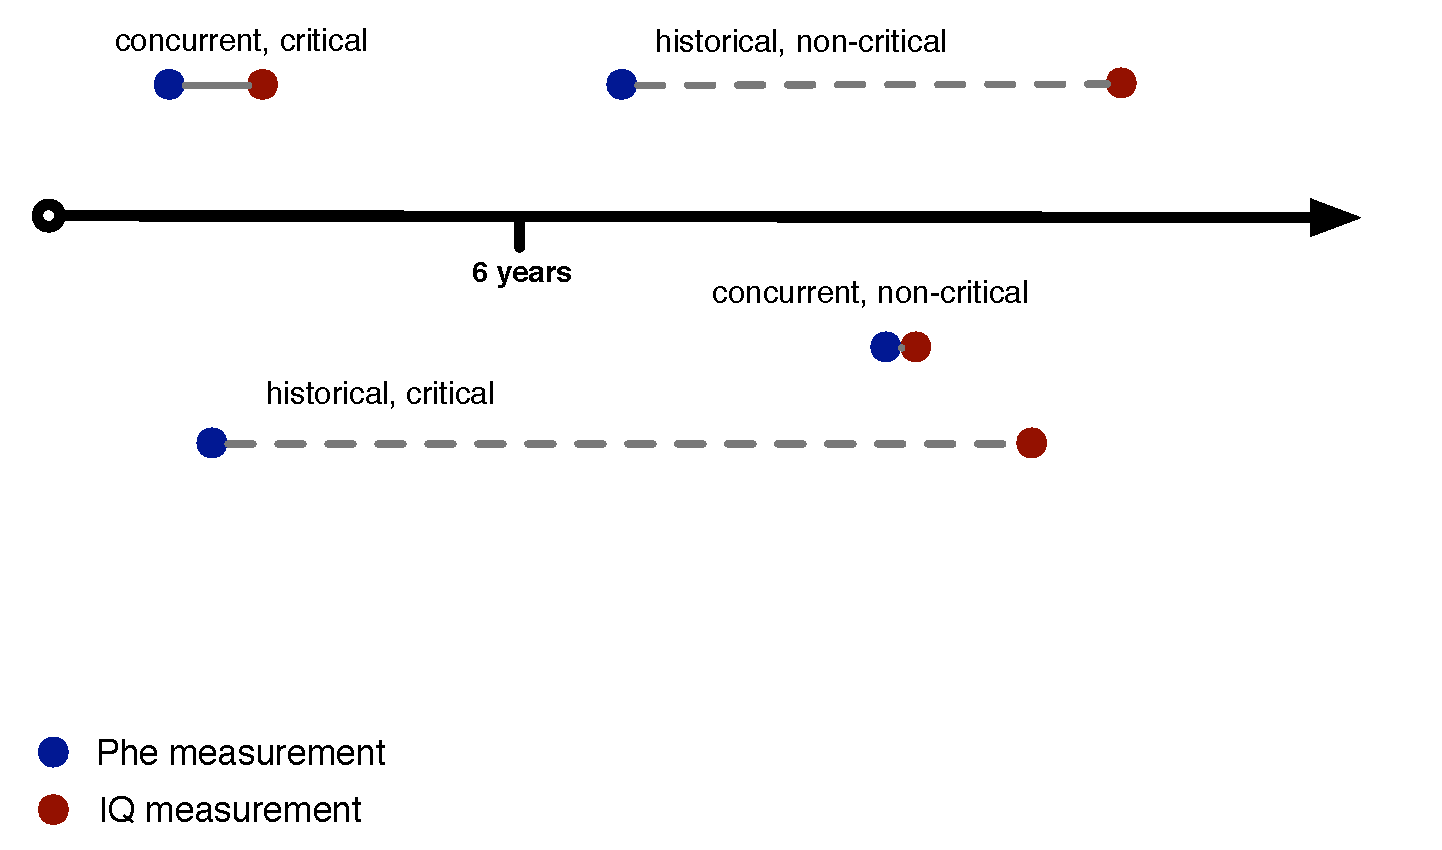
\includegraphics[width=\textwidth]{measurement.pdf}
    % 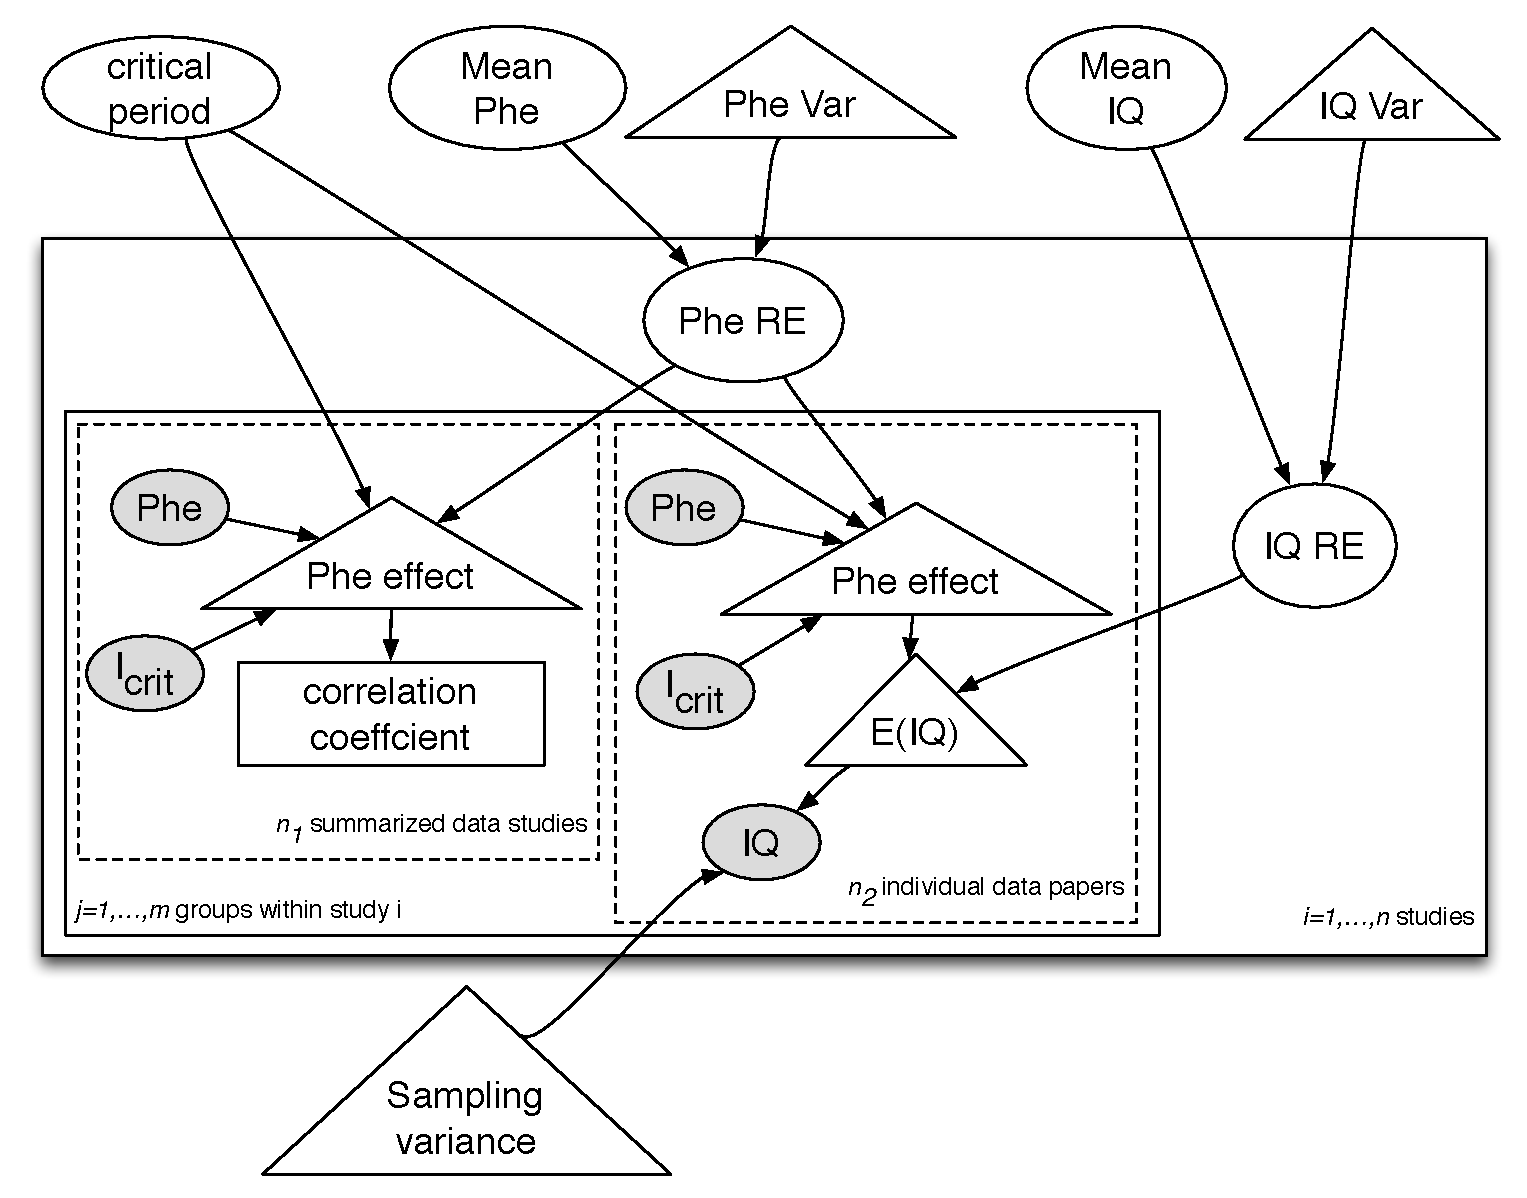
\includegraphics[width=0.5\textwidth]{model.pdf}

    % figure caption is below the figure
    \caption{Diagram illustrating the four possible scenarios of Phe and IQ measurement, depending on whether Phe was measured during the critical period and whether the corresponding IQ measurement was concurrent with Phe.} \label{fig:measurement}

    % Give a unique label
\end{figure}


% For one-column wide figures use
\begin{figure}[p]

    % Use the relevant command to insert your figure file.
    % For example, with the graphicx package use

    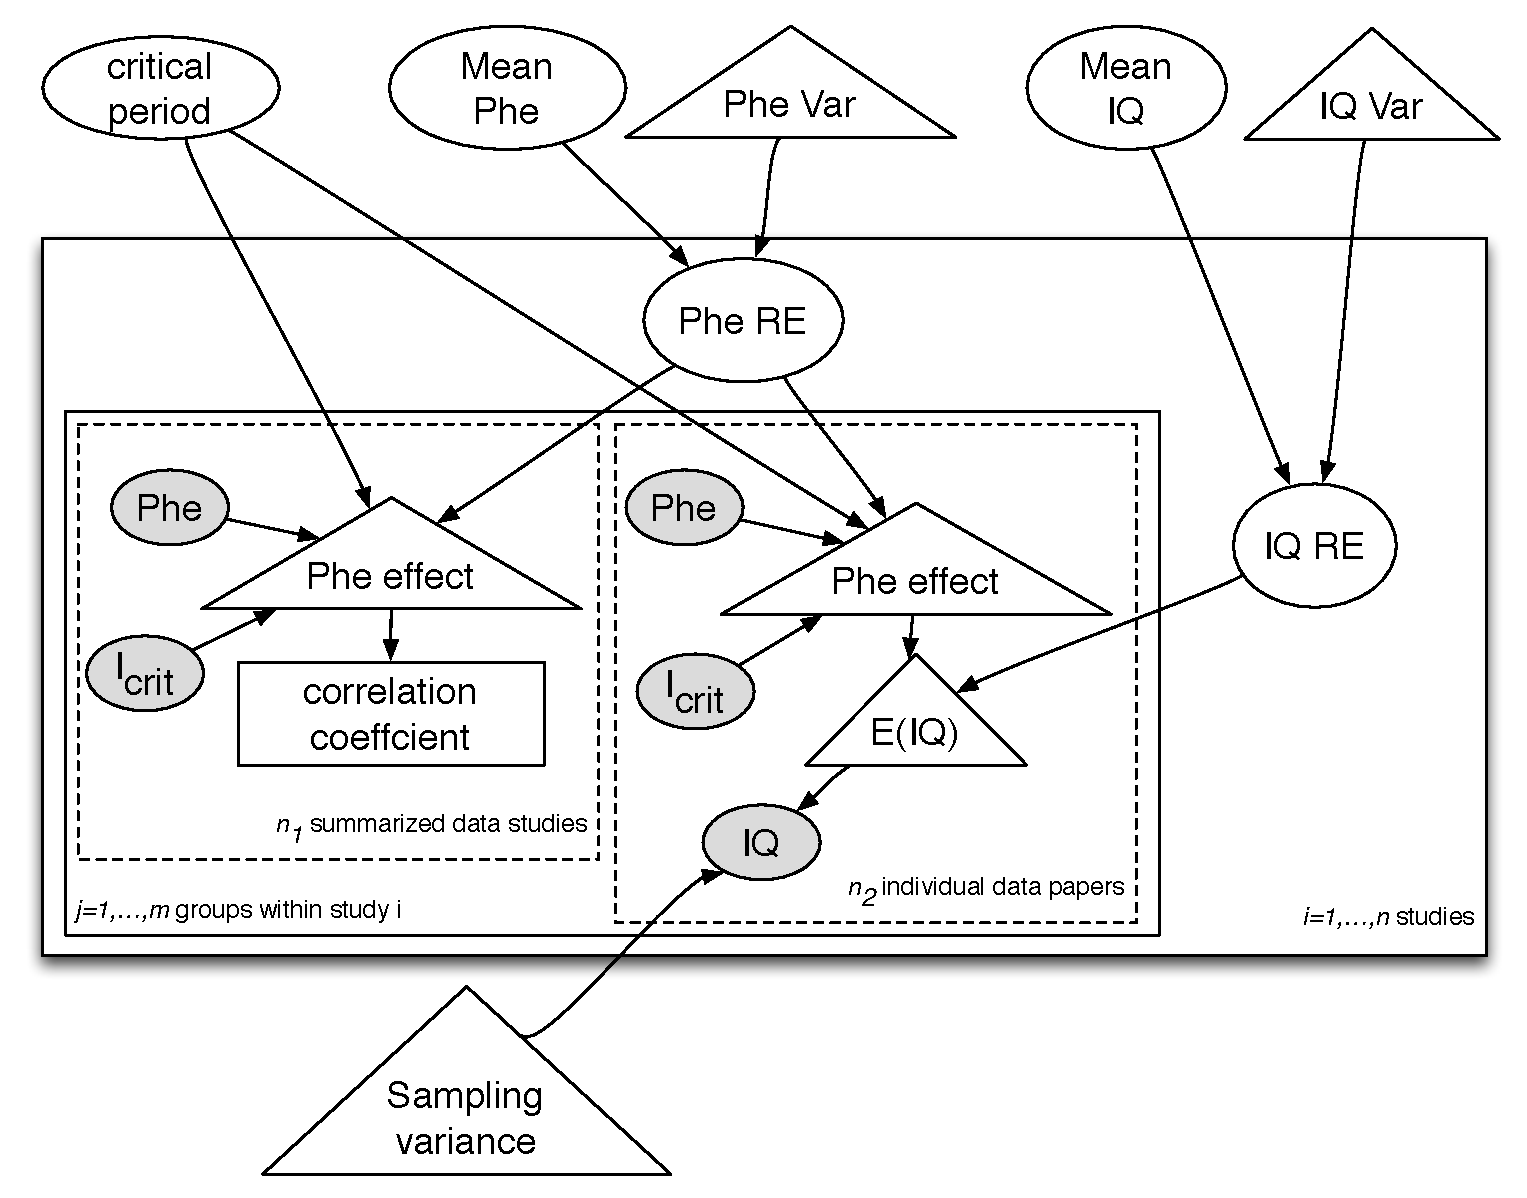
\includegraphics[width=\textwidth]{model.pdf}
    % 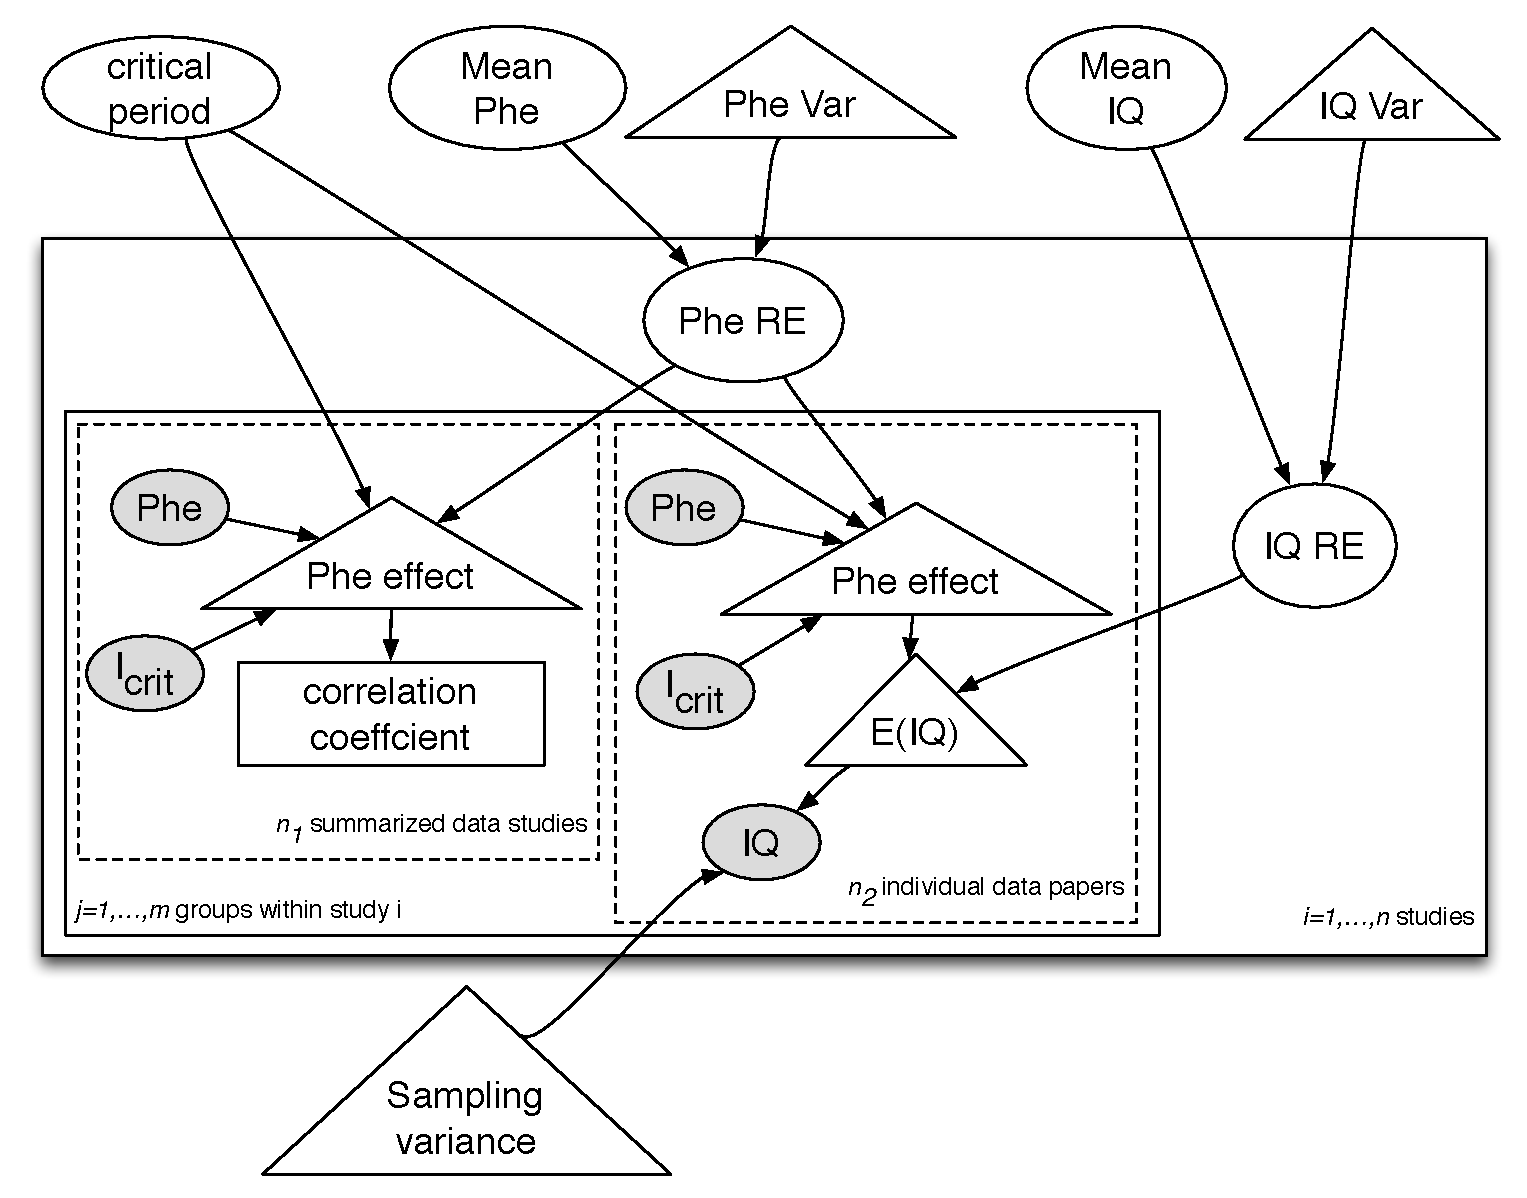
\includegraphics[width=0.5\textwidth]{model.pdf}

    % figure caption is below the figure
    \caption{Directed acyclic graph (DAG) showing the meta-analysis model structure, which is used for both the concurrent and historical Phe measurement models. Unfilled circles represent stochastic nodes (RE = random effect), shaded circles represent data, triangles represent deterministic nodes and squares represent factor potentials (arbitrary log-probability terms). The large enclosing square represents the collection of n unique studies in the meta-analysis; the smaller enclosing box represents the distinct groups (\emph{i.e.} subsets that had distinct covariates) within each study. Different information was contributed depending on whether the study provided group-summarized data ($n_1$ studies) or individual-level data ($n_2$ studies), as indicated by the dashed boxes; group-level data provided inference on the slope parameter only, while individual-level data informed both the slope and intercept. The data node $I_{crit}$ is an indicator variable that equals one for studies with Phe measurements in the critical period, and zero otherwise.} \label{fig:model}

    % Give a unique label
\end{figure}

\begin{figure}[p]
    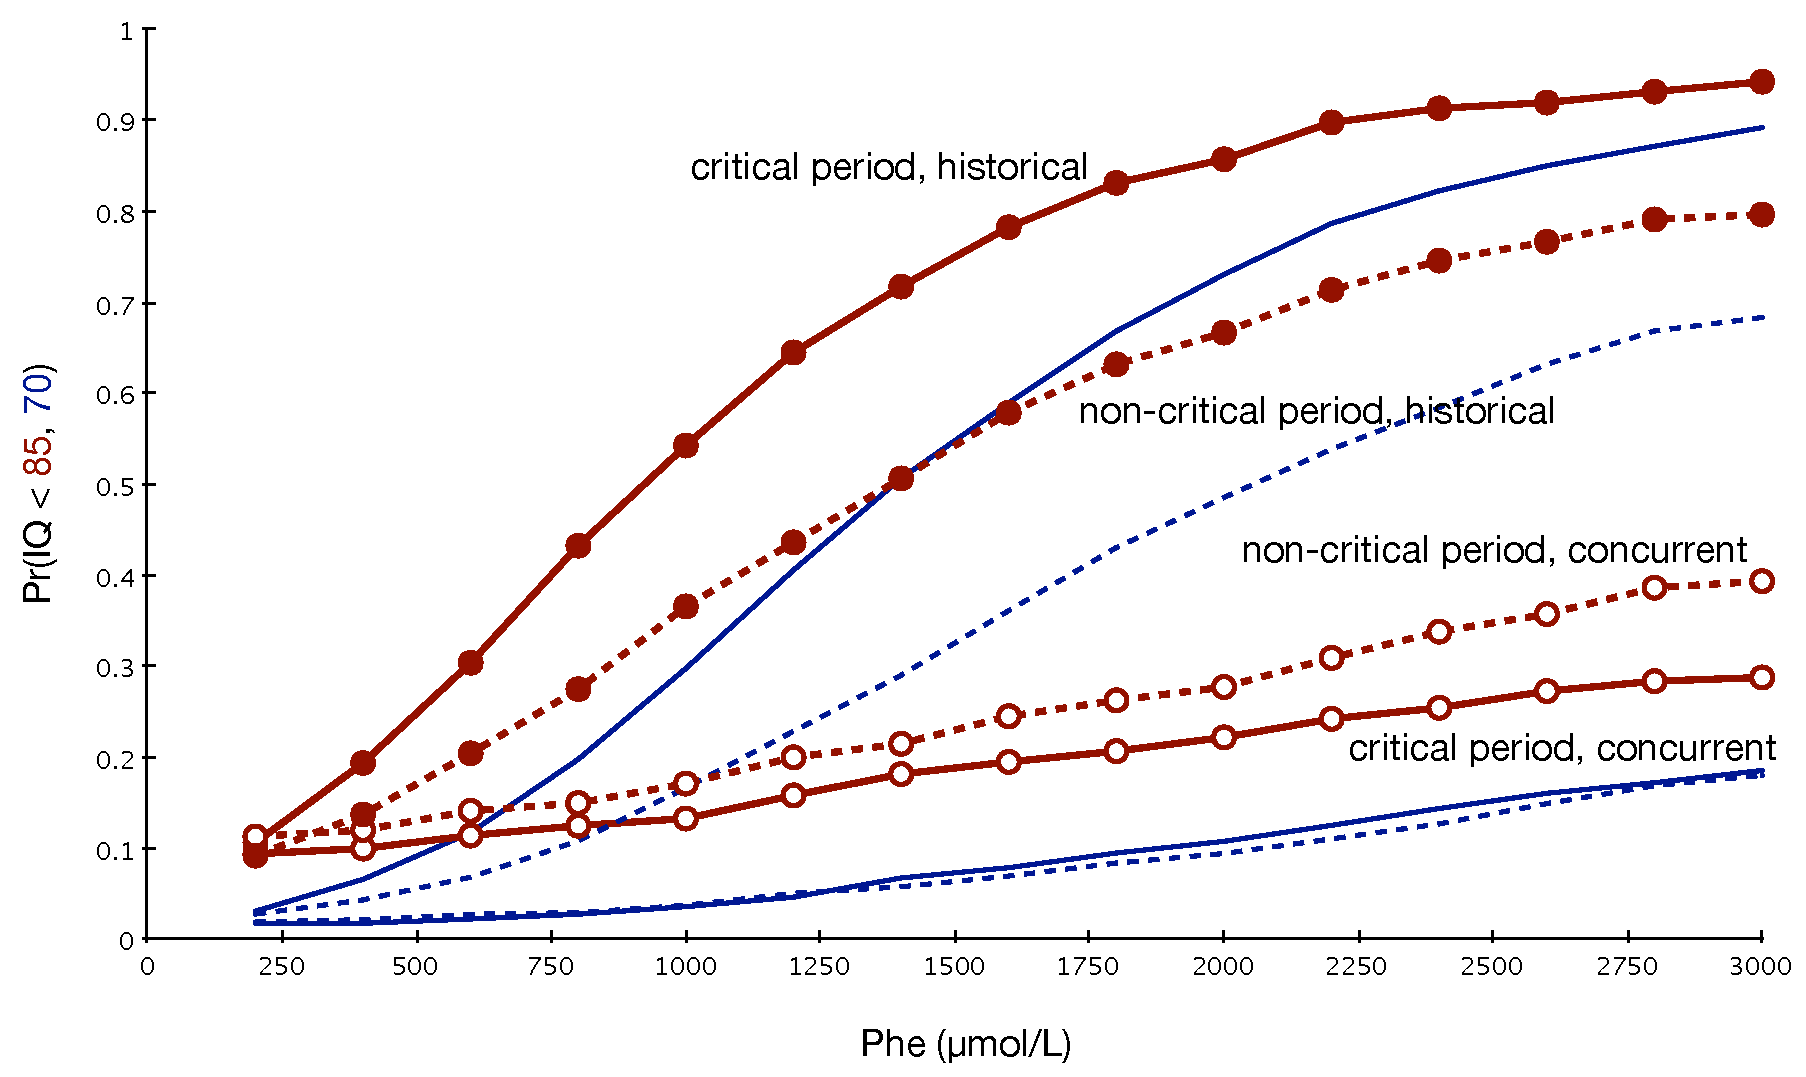
\includegraphics[width=\textwidth]{figure.pdf}

    \caption{Probability of IQ $<85$ (dark lines) at varying blood Phe levels and Phe measurement times. Solid lines represent critical period Phe measurements and dashed lines represent measurements outside the critical period. In addition, historical measurements are represented by red lines, concurrent measurements by blue. Corresponding lighter lines, using the same line style, represent the probability of IQ $<70$. The predictive region that extrapolates beyond the range of data provided by the studies in the meta-analysis is shaded gray.} \label{fig:probs}
    % \caption{Probability of IQ $<85$ at varying blood Phe levels and Phe measurement times. Solid lines represent critical perod Phe measurements and dashed lines represent measurements outside the critical period. Historical measurements are represented by solid circles, concurrent measurements by open circles.} \label{fig:probs}
\end{figure}


\begin{acknowledgements}
The authors would like to acknowledge the contributions of M. Bauer, J. Fisher, K. Jackson, R. Jerome, S. Jones, K. Lee, N. Sathe, T. Shields and Y. Summers, each of whom contributed importantly to the systematic review.
\end{acknowledgements}

\appendix
\section{Supplementary materials} % (fold)
\label{sec:Supplementary materials}

Supplementary materials, including model source code and data, are available at \url{http://github.com/fonnesbeck/PKUMetaAnalysis}.

% section Supplementary materials (end)

\section{Abbreviations} % (fold)
\label{sec:abbreviations}
\begin{itemize}
    \item[\textbf{BCI}] Bayesian credible interval
    \item[\textbf{E}] Expected value
    \item[\textbf{IQ}] Intelligence quotient
    \item[\textbf{MCMC}] Markov chain Monte Carlo
    \item[\textbf{Phe}] Phenylalanine
    \item[\textbf{PKU}] Phenylketonuria
    \item[\textbf{RE}] Random effect
    \item[\textbf{SD}] Standard deviation
\end{itemize}
% section abbreviations (end)

% BibTeX users please use one of
\bibliographystyle{spbasic}

% basic style, author-year citations
%\bibliographystyle{spmpsci}      % mathematics and physical sciences
%\bibliographystyle{spphys}       % APS-like style for physics
\bibliography{refs}

% name your BibTeX data base
\end{document}